\documentclass{article}
\usepackage[]{color}

\usepackage{hyperref} % Almost certainly will need
\usepackage{fullpage} % Good for making PDFs as well
\usepackage{listings} % Needed to insert code
\usepackage{lstautogobble}
\usepackage{float}

\usepackage{graphicx}
\usepackage{textcomp}
\usepackage[T1]{fontenc}
% This makes it so the web pages don't have indents as most of the time
% they are just annoying
\setlength{\parindent}{0pt}
% Makes code in lstlisting copy-and-paste-able
\lstset{
  upquote=true,
  basicstyle = \ttfamily,
  columns=fullflexible
  escapeinside=||,
  autogobble
}
% --- This section allows for tex4ht only control statements
% From http://tex.stackexchange.com/questions/93852/what-is-the-correct-way-to-check-for-latex-pdflatex-and-html-in-the-same-latex
\makeatletter
\edef\texforht{TT\noexpand\fi
  \@ifpackageloaded{tex4ht}
    {\noexpand\iftrue}
    {\noexpand\iffalse}}
\makeatother

\newcommand{\code}[1]{\texttt{\textmd{#1}}}

\newif\ifComments
%\Commentstrue
\ifComments
\newcommand{\nelson}[1]{\noindent\textcolor{red}{Nelson: {#1}}}
\newcommand{\marcus}[1]{\noindent\textcolor{blue}{Marcus {#1}}}
\else
\newcommand{\nelson}[1]{}
\newcommand{\marcus}[1]{}
\fi


\begin{document}

% This is an example of using a switch to have pdf/html only code
\ifpdf
	\LARGE
	\textbf{Generator Assignment}
	\normalsize
\fi


For this assignment you will be building a simple parser for a number generator. The generator will produce a series of
numbers. Your task is to parse the generator statement, interpret it, and print the numbers that should be produced by
the generator. You will be using \textit{Antlr4} to generate the \textbf{lexer} and \textbf{parser} for it. You will
then implement a interpreter in Java. Documentation and tutorials for \textit{Antlr4} can be found here 
\href{https://github.com/antlr/antlr4/blob/master/doc/index.md}
{Antlr4 documentation}


\section{Language Specification}

	\subsection{Generator}
		A generator generates a series of numbers based on an expression and bounds.  In a sense it is similar to a
		\textit{C} style \code{for} loop. \nelson{I think that the following sentences are ambiguous. Also I think that this is too early to make this spec, see below.} For this assignment generators will always start at the lower bound and continue
		until they are equal to the upper bound \textit{(It will continue until it is greater than the upper bound)}. The
		generator will always increment by the integer value 1.
                 
	\subsubsection{Generator format}
		The generator format will always follow the same format
		
		\begin{lstlisting}
			[ <id> in <int_1>..<int_2> | <expr>];
		\end{lstlisting}

		\begin{itemize}
			\item{\code{<id>}} is the identifier of a variable.
			\item{\code{<int\_1>}} is an integer representing the lower bound of the generator
			\item{\code{<int\_2>}} is an integer representing the upper bound of the generator
			\item{\code{<expr>}} is an expression
		\end{itemize}

\nelson{Is this what you meant to say?\\}
                 For this assignment the value of the identifier variable \code{<id>} is initialized to the value of \code{<int\_1>}, it is incremented by one until the value is equal \code{<int\_2>}. For each value assumed by \code{<id>}, \code{<expr>} is evaluated to generate each of the numbers in the series of numbers.
		
		\textbf{Assertion:} Your solution can assume that \code{<int\_1>} is less than or equal to \code{<int\_2>}
		
		Examples of valid generators:

		\begin{lstlisting}
			[i in 1..10 | i * i];
			
			[i in 0..10 | 2 ^ i];
		\end{lstlisting}

		In this assignment white space is not important so the following is valid:

		\begin{lstlisting}
			[i
			in
			1
			..
			10
			|
			i*i];
			[i in 1..10|2^i];
		\end{lstlisting}

		Because identifiers need white space to separate each other the following is invalid:

		\begin{lstlisting}
			[iin1..10|i*i];
			[i in1..10|2^i];
		\end{lstlisting}


	\subsection{Identifier}
		For the purpose of this assignment identifiers are simple. They must start with a character followed by
		numbers and characters.
		
		Examples of valid identifiers:

		\begin{lstlisting}
			hello
			h3llo
			Hi
			h3
		\end{lstlisting}

		Examples of invalid identifier:

		\begin{lstlisting}
			3d
			a-bad-variable-name
			no@twitter
			we.don't.like.punctuation
			or_spelling
		\end{lstlisting}

		there is only one key word \texttt{in}. This means that it is an invalid ID and should not be used as an ID.


	\subsection{Integers}

		In this assignment integers are defined as being a string that contains only the number characters 0-9 with no
		spaces. For the purpose of simplicity all integers in \textbf{input} are positive and can fit in a 32-bit signed integer representation.
		
		Examples of valid integers:

		\begin{lstlisting}
			1
			123
			5234
			01
			10
		\end{lstlisting}

		Examples of invalid integers:

		\begin{lstlisting}
			1.0
			one
			1_1
			1o
			4294967296
		\end{lstlisting}


	\subsection{Expression}

		An expression is composed of integers, identifiers, and integer mathematical operations.  Valid formats for
		expressions are

		\begin{lstlisting}
			<id>
			<int>
			(<expr>)
			<expr> <op> <expr>
		\end{lstlisting}

		\begin{itemize}
			\item{<id>} is the identifier of a variable
			\item{<int>} is an integer
			\item{<expr>} is an expression
		\end{itemize}
		
		An Example of valid expressions are

		\begin{lstlisting}
			i * 2 * 10 + 4
			2 ^ 4 * 5
		\end{lstlisting}
		
		\begin{center}
			\begin{tabular}{|l|c|l|c|}
				\hline
				\textbf{Operation} & \textbf{Symbol} & \textbf{Usage} &
				\textbf{Associativity} \\
				\hline
					addition       & +  & \code{expr + expr}  & left \\
					subtraction    & -  & \code{expr - expr}  & left \\
					multiplication & *  & \code{expr * expr}	& left \\
					division       & /  & \code{expr / expr}	& left \\
					modulus        & \% & \code{expr \% expr}	& left \\
					exponentiation & \textasciicircum & \code{expr \textasciicircum\ expr} & right\\
				\hline
			\end{tabular}
		\end{center}


	\subsubsection{Precedence}
	
		Precedence determines what order operations are evaluated in. Precedence works as defined in the following
		table:
		
		\begin{center}
			\begin{tabular}{|c|c|}
			\hline
			\textbf{Precedence} & \textbf{Operations} \\
			\hline
			HIGHER
			& \textasciicircum \\
			& *,/,\% \\
			LOWER & +,- \\
			\hline
			\end{tabular}
		\end{center}
		
		
		The higher the precedence the sooner the value should be evaluated. For example in the expression

		\begin{lstlisting}
		1 + 2 * 3
		\end{lstlisting}
		
		\code{2 * 3} should be evaluated before \code{1 + 2}. This is because multiplication, division, and modulus
		have higher precedence that addition and subtractions.


	\subsubsection{Associativity} % TODO Finish this section

		When parsing expressions associativity determines in what order operators of the same precedence should be
		evaluated in. For example:
		
		\begin{lstlisting}
			1 / 2 * 3
		\end{lstlisting}
		
		In this example both division and multiplication have the same precedence this is where associativity is
		important.  Left associative operations will form a parse tree like this:
		
		\begin{figure}[h]
			\centering
			
\includegraphics{static/left-assoc-gen.png}
		\end{figure}
		
		An example of one of these operations is addition. Lets say we have the following expression:
		
		\begin{lstlisting}
			1 + 2 + 3 + 4
		\end{lstlisting}
		
		Because addition is left associative it will form the following parse tree:
		
		\begin{figure}[H]
			\centering
			
\includegraphics{static/left-assoc-plus.png}
		\end{figure}
		
		In parse trees evaluation can only happen when there are on only leaves as children. So it will evaluate
		\code{1 + 2}. The result of this will be pushed up and the following tree will be created.
		
		\begin{figure}[H]
			\centering
			
\includegraphics{static/left-assoc-plus-2.png} after that \code{3 + 3} are evaluated making
			
\includegraphics{static/left-assoc-plus-3.png}
		\end{figure}
		
		Most operations used in this assignment are left associative \textit{see table operation table for more info}
		but there also exist operations that are right associative and take the format
		
		\begin{figure}[H]
			\centering
			
\includegraphics{static/right-assoc-gen.png}
		\end{figure}
		
		An example of a right associative operation is the power symbol or
		
		\code{\textasciicircum}. For example:
		
		\begin{lstlisting}
			2 ^ 3 ^ 4 ^ 5
		\end{lstlisting}
		
		should be evaluated like so:
		
		\begin{math}
			2 ^ {\displaystyle 3 ^ {\displaystyle 4 ^ {\displaystyle 5 }}}
		\end{math}
		
		In order for this expression to be evaluated correctly the following parse tree must be generated
		
		\begin{figure}[H]
			\centering
			
\includegraphics{static/right-assoc-pow.png}
		\end{figure}
		
		For a more complex example let's take the expression:
		
		\begin{lstlisting}
		1 + 2 * 3 + 1 / 3 ^ 4 ^ (6 * 3)
		\end{lstlisting}
		
		This should generate the following parse tree:
		
		\begin{figure}[H]
			\centering
			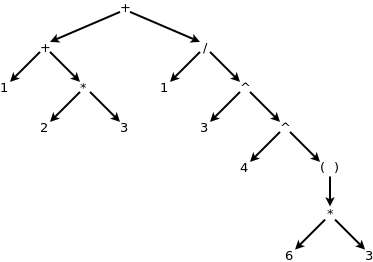
\includegraphics{static/assoc-example.png}
		\end{figure}


\section{Output}
	
	Output will have a very specific format to allow easy marking All the numbers generated by the generator will be
	printed on the same line with spaces separating each number. There should be a new line after each generator's
	output. 
	
	Example input:
	
	\begin{lstlisting}
		[i in 1..10| i];
		[x in 0..3| x-1];
		[x in 1..4| 10];
	\end{lstlisting}
	
	Expected Output:
	
	\begin{lstlisting}
		1 2 3 4 5 6 7 8 9 10
		-1 0 1 2
		10 10 10 10
	\end{lstlisting}


\section{Provided Frameworks}

	The following tools have been provided for you to make development and testing easier 

	\subsection{Project Layout}
	
		For the tools provided to work your project should be in the specified layout.
		
		\begin{lstlisting}
			+-- project/
				+-- README
				+-- Makefile
				+-- genertor_tester
				+-- src/
					+-- Main.java	(must contain main function)
					+-- *.g4		(Antlr4 lexer/parser source files)
					+-- *.java		(Java source files)
				+-- TestFiles/
					+-- Input/
						+-- (testfiles)
						+-- test_01
						+-- test_02
						+-- ...
					+-- Output/
						+-- (matching output files. Names must match between input test and output test)
						+-- test_01
						+-- test_02
						+-- ...
		\end{lstlisting}


	\subsection{Makefile}
	
		The \texttt{Makefile} provided is an exact copy of the one that will be used for grading.  Any changes made to
		this makefile will not exist in the one used for grading so as a rule of thumb don't change it. The project must
		be in the specified layout for the makefile to properly work (see \texttt{Project Layout})
		
		The makefile has the following commands:
		
		\begin{itemize}
			\item{\textbf{all}}: Builds all solution files
			\item{\textbf{run}}: Runs the solution (builds solution if necessary) takes f="<filename>" as an argument for
				input file
			\item{\textbf{test}}: Runs testing system against solution (builds solution if necessary)
			\item{\textbf{clean}}: Cleans all generated files including IntelliJ generated files
			\item{\textbf{submissible}}: Collects files for submission and places them in a tar ball. This file contains
			the files in the format they should be in
		\end{itemize}

	\subsection{generator\_tester}
	
		This program runs all your test files against their matching outputs. This program is designed to operate in the
		same manor as how the marking script will test solutions. For best results have \textit{colordiff} installed.
		
		Help for generator tester can be found by running with the -h flag:
		
		\begin{lstlisting}
			./generator_tester -h
		\end{lstlisting}
		
		It by default expects that all input Tests are in \texttt{TestFiles/Input/} and that  all output files are in
		\texttt{TestFiles/Output/}

\section{Deliverables}

	To prepare your project for delivery use the Makefile provided and use the \texttt{submissible} command. Ex:
	
	\begin{lstlisting}
		make submissible
	\end{lstlisting}
	
	The makefile will prompt you to enter your CCID (not your student id number). This should create a file called:
	
	\begin{lstlisting}
		submission_<CCID>.tar.gz
	\end{lstlisting}

	This submission file will contain your \texttt{src} folder, \texttt{TestFiles}, and your README
	\begin{lstlisting}
		+-- submission_<CCID>.tar.gz
			+-- README
			+-- src/
				+--	Main.Java
				+-- *.g4
				+-- *.Java
			+-- TestFiles/
				+-- Input/
					+-- (testfiles)
					+-- test_01
					+-- test_02
					+-- ...
				+-- Output/
					+-- (matching output files. Names must match between input test and output test)
					+-- test_01
					+-- test_02
					+-- ...
		\end{lstlisting}


\section{Tips and Hints}
	
	\begin{enumerate}
		\item Write tests \textbf{BEFORE} you implement the things they will test. The testing script provide is
		designed to handle failed test cases. You can turn off stopping on invalid output and you can also turn off
		displaying erroneous output with the flags "-a and -s" respectively.
		\item First and foremost \textbf{READ THE DOCUMENTATION FOR ANTLR4} here is the link again
			\href 
			{https://github.com/antlr/antlr4/blob/master/doc/index.md}
			{Antlr4 documentation}.
		\item \textit{Antlr4} has two ways of navigating the parse tree, Visitors and Listeners. For this assignment use the
			visitor method. For the next assignment you'll use either but for this assignment the visitor is better
			suited.
		\item Remember that in the lexer the order of when tokens are defined is very important. The lexer will try to
			follow the first rule it can.
		\item \textit{Antlr4} has no standardized naming convention or style guide. This means you \textbf{CAN} do whatever you
			want for style. With that in mind I highly recommend you follow something similar to the one on the \textit{Antlr4}
			documentation pages. What ever you choose make sure it is easy to read and is consistent as \textbf{part of
			your grade} will be based of your software design and that includes code legibility.
	\end{enumerate}

\end{document}
